\section{Introduction}
% =========================================
% =========================================




\begin{frame}{Introduction}
	\framesubtitle{Handbooks and references}
	UUV - Unmanned Underwater vehicle
	\begin{figure}
		\centering
		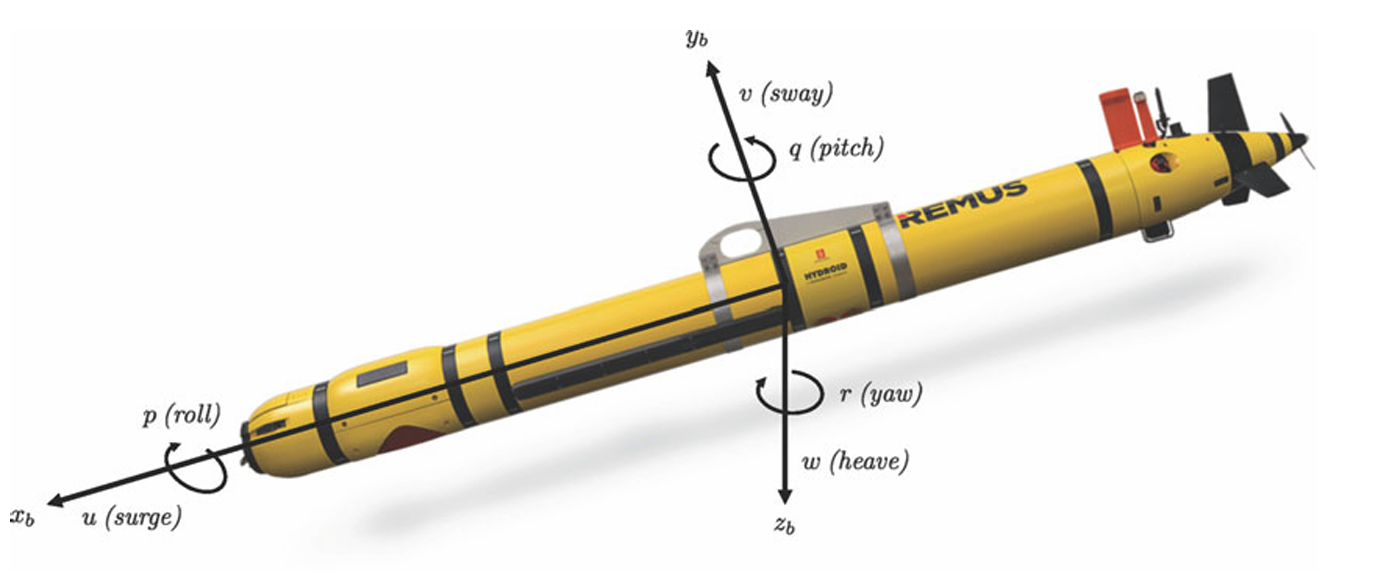
\includegraphics[width=0.75\linewidth]{img/6DOF motion AUV}
		\caption{6-DOF motion variables for a UUV/AUV}
		\label{fig: UUV}
	\end{figure}
	
	Handbooks \& References:
	\begin{itemize}
		\item Thor I. Fossen, \textit{Handbook of Marine Craft Hydrodynamics and Motion Control}, Wiley, 2011.
		\item Thor I. Fossen, \textit{Guidance and Control of Ocean Vehicles}, Wiley, 1994.
	\end{itemize}
	
\end{frame}

% =========================================
% =========================================




\begin{frame}{Introduction}
	\framesubtitle{Handbooks and references}
	\begin{tikzpicture}[remember picture,overlay]
		% \node[fill=blue!30, text=white, font=\large, rounded corners] 
		\node at (current page.north east) [xshift=-11cm, yshift=-3.5cm] 
		{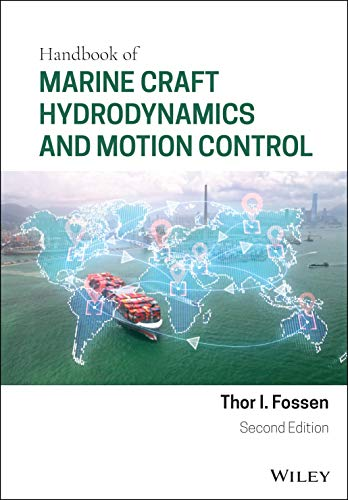
\includegraphics[width=0.23\linewidth]{img/handbook.png}};
	\end{tikzpicture}
	
	\begin{tikzpicture}[remember picture,overlay]
		% \node[fill=blue!30, text=white, font=\large, rounded corners] 
		\node at (current page.north east) [xshift=-8cm, yshift=-3.5cm] 
		{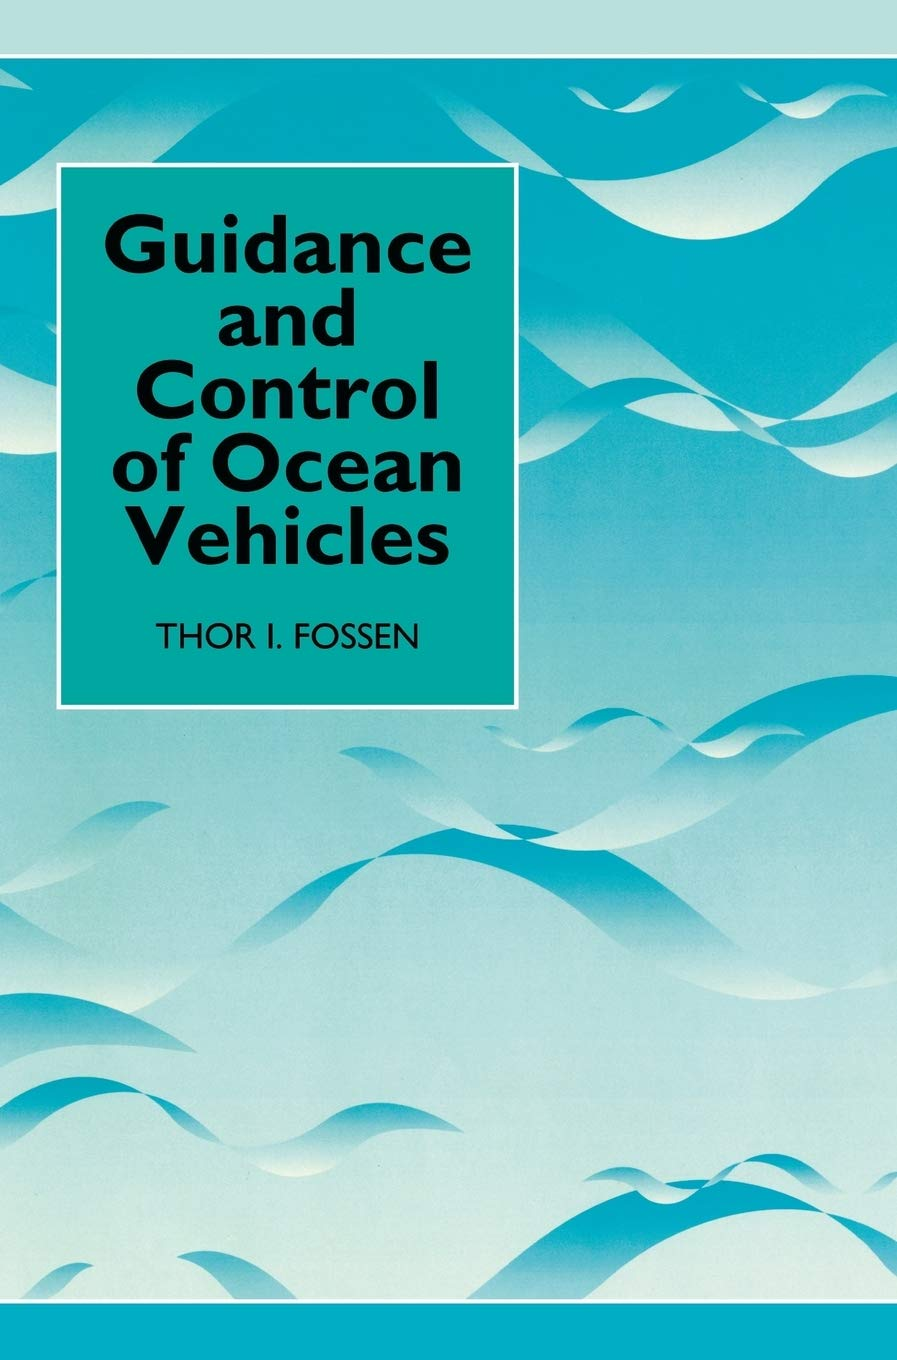
\includegraphics[width=0.23\linewidth]{img/handbook1.png}};
	\end{tikzpicture}
	
	\begin{tikzpicture}[remember picture,overlay]
		% \node[fill=blue!30, text=white, font=\large, rounded corners] 
		\node at (current page.north east) [xshift=-5cm, yshift=-3.5cm] 
		{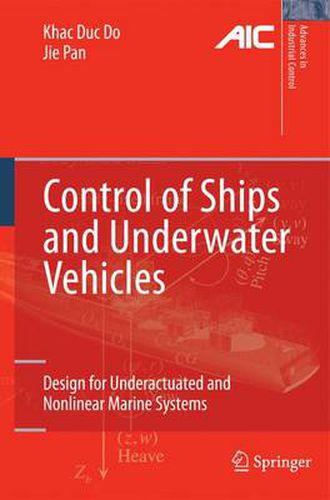
\includegraphics[width=0.23\linewidth]{img/handbook2.png}};
	\end{tikzpicture}
	
	\begin{tikzpicture}[remember picture,overlay]
		% \node[fill=blue!30, text=white, font=\large, rounded corners] 
		\node at (current page.north east) [xshift=-2cm, yshift=-3.5cm] 
		{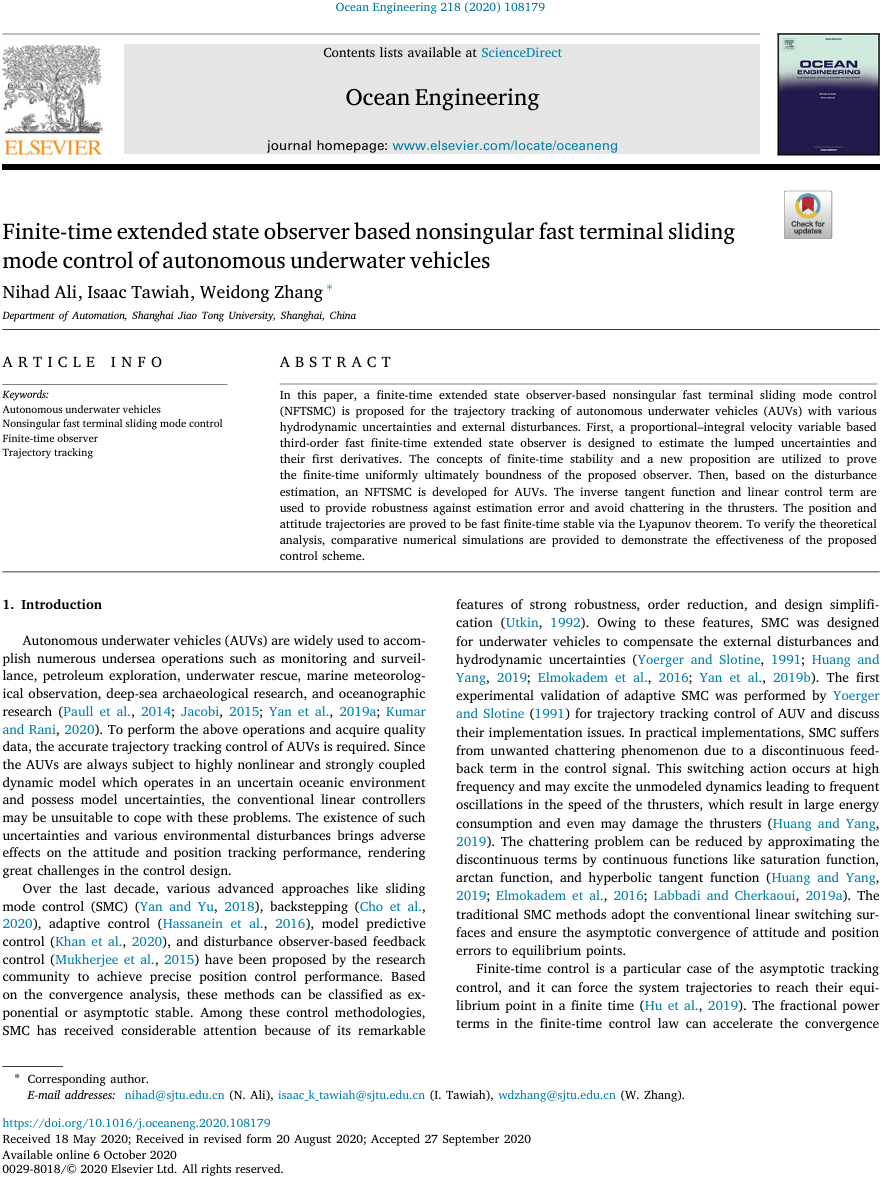
\includegraphics[width=0.23\linewidth]{img/handbook4.png}};
	\end{tikzpicture}
	
	
	
	\vspace{2cm}
	
	Handbooks \& References:
	\begin{itemize}
		\item Review articles, Research articles, Handbook, ...
		\item IEEE Explore, Springer, Elserview, Wiley, Taylor \& Francis, ...
	\end{itemize}
	
\end{frame}

% =========================================
% =========================================




\begin{frame}{Introduction}
	\framesubtitle{Automatic Weather Routing}
	\centering
	\scalebox{0.8}{

\tikzset{every picture/.style={line width=0.75pt}} %set default line width to 0.75pt        

\begin{tikzpicture}[x=0.75pt,y=0.75pt,yscale=-1,xscale=1]
%uncomment if require: \path (0,400); %set diagram left start at 0, and has height of 400

%Rounded Rect [id:dp024716399980995396] 
\draw  [fill={rgb, 255:red, 126; green, 211; blue, 33 }  ,fill opacity=0.63 ][dash pattern={on 4.5pt off 4.5pt}] (224.86,72.14) .. controls (224.86,61.32) and (233.63,52.55) .. (244.44,52.55) -- (558.6,52.55) .. controls (569.42,52.55) and (578.19,61.32) .. (578.19,72.14) -- (578.19,130.9) .. controls (578.19,141.72) and (569.42,150.49) .. (558.6,150.49) -- (244.44,150.49) .. controls (233.63,150.49) and (224.86,141.72) .. (224.86,130.9) -- cycle ;
%Rounded Rect [id:dp820569210963702] 
\draw  [fill={rgb, 255:red, 74; green, 144; blue, 226 }  ,fill opacity=0.71 ][dash pattern={on 4.5pt off 4.5pt}] (104.19,178.89) .. controls (104.19,170.2) and (111.23,163.16) .. (119.92,163.16) -- (443.79,163.16) .. controls (452.48,163.16) and (459.52,170.2) .. (459.52,178.89) -- (459.52,226.09) .. controls (459.52,234.78) and (452.48,241.82) .. (443.79,241.82) -- (119.92,241.82) .. controls (111.23,241.82) and (104.19,234.78) .. (104.19,226.09) -- cycle ;
%Rounded Rect [id:dp6482229762233973] 
\draw  [color={rgb, 255:red, 0; green, 0; blue, 0 }  ,draw opacity=1 ][fill={rgb, 255:red, 208; green, 2; blue, 27 }  ,fill opacity=0.38 ][dash pattern={on 4.5pt off 4.5pt}] (102.86,271.08) .. controls (102.86,261.22) and (110.86,253.22) .. (120.72,253.22) -- (472.32,253.22) .. controls (482.19,253.22) and (490.19,261.22) .. (490.19,271.08) -- (490.19,324.68) .. controls (490.19,334.55) and (482.19,342.55) .. (472.32,342.55) -- (120.72,342.55) .. controls (110.86,342.55) and (102.86,334.55) .. (102.86,324.68) -- cycle ;
%Shape: Rectangle [id:dp008171136473899221] 
\draw   (367.33,88.67) -- (437.33,88.67) -- (437.33,128.67) -- (367.33,128.67) -- cycle ;
%Shape: Rectangle [id:dp578249717098626] 
\draw   (487.67,78.33) -- (557.67,78.33) -- (557.67,118.33) -- (487.67,118.33) -- cycle ;
%Shape: Rectangle [id:dp05994207844147015] 
\draw   (246,88.67) -- (316,88.67) -- (316,128.67) -- (246,128.67) -- cycle ;
%Shape: Rectangle [id:dp3752897955760164] 
\draw   (368.67,183.83) -- (438.67,183.83) -- (438.67,223.83) -- (368.67,223.83) -- cycle ;
%Shape: Rectangle [id:dp9144008780653681] 
\draw   (130.67,183.83) -- (200.67,183.83) -- (200.67,223.83) -- (130.67,223.83) -- cycle ;
%Shape: Rectangle [id:dp6067520460647975] 
\draw   (261.33,183.83) -- (331.33,183.83) -- (331.33,223.83) -- (261.33,223.83) -- cycle ;
%Shape: Rectangle [id:dp21504321988161568] 
\draw   (356,259.33) -- (452,259.33) -- (452,299.33) -- (356,299.33) -- cycle ;
%Shape: Rectangle [id:dp2963684683337764] 
\draw   (239.33,259.33) -- (309.33,259.33) -- (309.33,299.33) -- (239.33,299.33) -- cycle ;
%Shape: Rectangle [id:dp12173800355567699] 
\draw   (111.67,260) -- (181.67,260) -- (181.67,300) -- (111.67,300) -- cycle ;
%Straight Lines [id:da588131875954907] 
\draw    (164.19,183.88) -- (164.19,108.55) -- (244.86,108.55) ;
\draw [shift={(246.86,108.55)}, rotate = 180] [color={rgb, 255:red, 0; green, 0; blue, 0 }  ][line width=0.75]    (10.93,-3.29) .. controls (6.95,-1.4) and (3.31,-0.3) .. (0,0) .. controls (3.31,0.3) and (6.95,1.4) .. (10.93,3.29)   ;
%Straight Lines [id:da637808700504805] 
\draw    (316.47,109.33) -- (364.8,109.33) ;
\draw [shift={(366.8,109.33)}, rotate = 180] [color={rgb, 255:red, 0; green, 0; blue, 0 }  ][line width=0.75]    (10.93,-3.29) .. controls (6.95,-1.4) and (3.31,-0.3) .. (0,0) .. controls (3.31,0.3) and (6.95,1.4) .. (10.93,3.29)   ;
%Straight Lines [id:da38171557543802015] 
\draw    (437.13,98.67) -- (485.47,98.67) ;
\draw [shift={(487.47,98.67)}, rotate = 180] [color={rgb, 255:red, 0; green, 0; blue, 0 }  ][line width=0.75]    (10.93,-3.29) .. controls (6.95,-1.4) and (3.31,-0.3) .. (0,0) .. controls (3.31,0.3) and (6.95,1.4) .. (10.93,3.29)   ;
%Straight Lines [id:da7149208141383911] 
\draw    (437.47,116.67) -- (472.13,116.67) -- (472.13,192) -- (441.47,192) ;
\draw [shift={(439.47,192)}, rotate = 360] [color={rgb, 255:red, 0; green, 0; blue, 0 }  ][line width=0.75]    (10.93,-3.29) .. controls (6.95,-1.4) and (3.31,-0.3) .. (0,0) .. controls (3.31,0.3) and (6.95,1.4) .. (10.93,3.29)   ;
%Straight Lines [id:da9344395667032277] 
\draw    (558,99) -- (590.13,99) -- (590.13,213.33) -- (440.13,213.33) ;
\draw [shift={(438.13,213.33)}, rotate = 360] [color={rgb, 255:red, 0; green, 0; blue, 0 }  ][line width=0.75]    (10.93,-3.29) .. controls (6.95,-1.4) and (3.31,-0.3) .. (0,0) .. controls (3.31,0.3) and (6.95,1.4) .. (10.93,3.29)   ;
%Straight Lines [id:da7282910208505873] 
\draw    (590.13,213.33) -- (590.13,291.33) -- (454.13,291.33) ;
\draw [shift={(452.13,291.33)}, rotate = 360] [color={rgb, 255:red, 0; green, 0; blue, 0 }  ][line width=0.75]    (10.93,-3.29) .. controls (6.95,-1.4) and (3.31,-0.3) .. (0,0) .. controls (3.31,0.3) and (6.95,1.4) .. (10.93,3.29)   ;
%Straight Lines [id:da9182086877003304] 
\draw    (472.13,192) -- (472.13,271.33) -- (454.13,271.33) ;
\draw [shift={(452.13,271.33)}, rotate = 360] [color={rgb, 255:red, 0; green, 0; blue, 0 }  ][line width=0.75]    (10.93,-3.29) .. controls (6.95,-1.4) and (3.31,-0.3) .. (0,0) .. controls (3.31,0.3) and (6.95,1.4) .. (10.93,3.29)   ;
%Straight Lines [id:da9524515432659333] 
\draw    (355.33,278.67) -- (311.47,278.67) ;
\draw [shift={(309.47,278.67)}, rotate = 360] [color={rgb, 255:red, 0; green, 0; blue, 0 }  ][line width=0.75]    (10.93,-3.29) .. controls (6.95,-1.4) and (3.31,-0.3) .. (0,0) .. controls (3.31,0.3) and (6.95,1.4) .. (10.93,3.29)   ;
%Straight Lines [id:da02741576724077044] 
\draw    (238.8,278) -- (184.13,278) ;
\draw [shift={(182.13,278)}, rotate = 360] [color={rgb, 255:red, 0; green, 0; blue, 0 }  ][line width=0.75]    (10.93,-3.29) .. controls (6.95,-1.4) and (3.31,-0.3) .. (0,0) .. controls (3.31,0.3) and (6.95,1.4) .. (10.93,3.29)   ;
%Straight Lines [id:da49199432560322975] 
\draw    (111.8,278.67) -- (90.19,278.67) -- (90.19,202.49) -- (128.86,202.49) ;
\draw [shift={(130.86,202.49)}, rotate = 180] [color={rgb, 255:red, 0; green, 0; blue, 0 }  ][line width=0.75]    (10.93,-3.29) .. controls (6.95,-1.4) and (3.31,-0.3) .. (0,0) .. controls (3.31,0.3) and (6.95,1.4) .. (10.93,3.29)   ;
%Straight Lines [id:da16345135268080146] 
\draw    (368.8,202.67) -- (334.13,202.67) ;
\draw [shift={(332.13,202.67)}, rotate = 360] [color={rgb, 255:red, 0; green, 0; blue, 0 }  ][line width=0.75]    (10.93,-3.29) .. controls (6.95,-1.4) and (3.31,-0.3) .. (0,0) .. controls (3.31,0.3) and (6.95,1.4) .. (10.93,3.29)   ;
%Straight Lines [id:da3511077229754682] 
\draw    (261.52,203.33) -- (203.52,203.33) ;
\draw [shift={(201.52,203.33)}, rotate = 360] [color={rgb, 255:red, 0; green, 0; blue, 0 }  ][line width=0.75]    (10.93,-3.29) .. controls (6.95,-1.4) and (3.31,-0.3) .. (0,0) .. controls (3.31,0.3) and (6.95,1.4) .. (10.93,3.29)   ;

% Text Node
\draw (372,99.2) node [anchor=north west][inner sep=0.75pt]   [align=left] {{\normalfont\selectfont { Dynamics}}};
% Text Node
\draw (489.33,87.87) node [anchor=north west][inner sep=0.75pt]   [align=left] {{\normalfont\selectfont { Kinematics}}};
% Text Node
\draw (387,188.2) node [anchor=north west][inner sep=0.75pt]   [align=left] {\begin{minipage}[lt]{26.74pt}\setlength\topsep{0pt}
{\normalfont\selectfont { Motion}}
\begin{center}
{\normalfont\selectfont { Sensor}}
\end{center}

\end{minipage}};
% Text Node
\draw (268,193.53) node [anchor=north west][inner sep=0.75pt]   [align=left] {{\normalfont\selectfont { Observer}}};
% Text Node
\draw (138.33,193.87) node [anchor=north west][inner sep=0.75pt]   [align=left] {{\normalfont\selectfont {Controller}}};
% Text Node
\draw (252.33,99.2) node [anchor=north west][inner sep=0.75pt]   [align=left] {{\normalfont\selectfont { Actuators}}};
% Text Node
\draw (326,51.87) node [anchor=north west][inner sep=0.75pt]   [align=left] {{\normalfont\selectfont { Ocean disturbances}}};
% Text Node
\draw (112.33,270.2) node [anchor=north west][inner sep=0.75pt]   [align=left] {{\normalfont\selectfont { Trajectories}}};
% Text Node
\draw (214.67,315.53) node [anchor=north west][inner sep=0.75pt]   [align=left] {{\normalfont\selectfont { Weather}}};
% Text Node
\draw (249.67,264.87) node [anchor=north west][inner sep=0.75pt]   [align=left] {\begin{minipage}[lt]{36.02pt}\setlength\topsep{0pt}
{\normalfont\selectfont { Guidance }}
\begin{center}
{\normalfont\selectfont { sensor}}
\end{center}

\end{minipage}};
% Text Node
\draw (366.33,263.87) node [anchor=north west][inner sep=0.75pt]   [align=left] {\begin{minipage}[lt]{53.18pt}\setlength\topsep{0pt}
{\normalfont\selectfont { Kinematics \\ Transformation}}

\end{minipage}};
% Text Node
\draw (347.33,325.53) node [anchor=north west][inner sep=0.75pt]   [align=left] {{\normalfont\selectfont { Guidance and Navigation}}};
% Text Node
\draw (114.67,222.2) node [anchor=north west][inner sep=0.75pt]   [align=left] {{\normalfont\selectfont { Measurement and Control}}};
% Text Node
\draw (239.33,128.87) node [anchor=north west][inner sep=0.75pt]   [align=left] {{\normalfont\selectfont { Dynamics System and Modeling}}};
% Connection
\draw    (386.86,72.87) -- (399.28,93.49) ;
\draw [shift={(400.31,95.2)}, rotate = 238.95] [color={rgb, 255:red, 0; green, 0; blue, 0 }  ][line width=0.75]    (10.93,-3.29) .. controls (6.95,-1.4) and (3.31,-0.3) .. (0,0) .. controls (3.31,0.3) and (6.95,1.4) .. (10.93,3.29)   ;
% Connection
\draw    (375.19,72.87) -- (387.61,93.49) ;
\draw [shift={(388.64,95.2)}, rotate = 238.95] [color={rgb, 255:red, 0; green, 0; blue, 0 }  ][line width=0.75]    (10.93,-3.29) .. controls (6.95,-1.4) and (3.31,-0.3) .. (0,0) .. controls (3.31,0.3) and (6.95,1.4) .. (10.93,3.29)   ;
% Connection
\draw    (246,311.53) -- (259.13,296.38) ;
\draw [shift={(260.44,294.87)}, rotate = 130.91] [color={rgb, 255:red, 0; green, 0; blue, 0 }  ][line width=0.75]    (10.93,-3.29) .. controls (6.95,-1.4) and (3.31,-0.3) .. (0,0) .. controls (3.31,0.3) and (6.95,1.4) .. (10.93,3.29)   ;

\end{tikzpicture}
}
\end{frame}


% =========================================
% =========================================

\begin{frame}{Introduction}
	\framesubtitle{Model classifications}
	Degree of Freedom classifications under purpose
	\begin{itemize}
		\item 1 DOF $\to$ model can be used to design the forward speed controller and heading autopilots and damping system
		\item 3 DOFs $\to$ describe the horizontal plane, longitudinal, and lateral models.
		\item 4 DOFs $\to$ describe the motion in the horizontal plane with heading autopilots and system damping
		\item 6 DOFs $\to$ describe the fully coupled equation of motion used for simulation and prediction.
	\end{itemize}
	
	Naval Architecture
	\begin{itemize}
		\item Maneuvering theory: moving at positive constant speed in calm water
		\item  Seeking theory: motion of ships at zero or constraint speed in waves, which can be analyzed. The hydrodynamic coefficient and wave forces are computed as a function
	\end{itemize}
\end{frame}

% =========================================
% =========================================

\begin{frame}{Introduction}
	\framesubtitle{Tools and Toolboxs}
	\begin{tikzpicture}[remember picture,overlay]
		% \node[fill=blue!30, text=white, font=\large, rounded corners] 
		\node at (current page.north east) [xshift=-4.5cm, yshift=-3cm] 
		{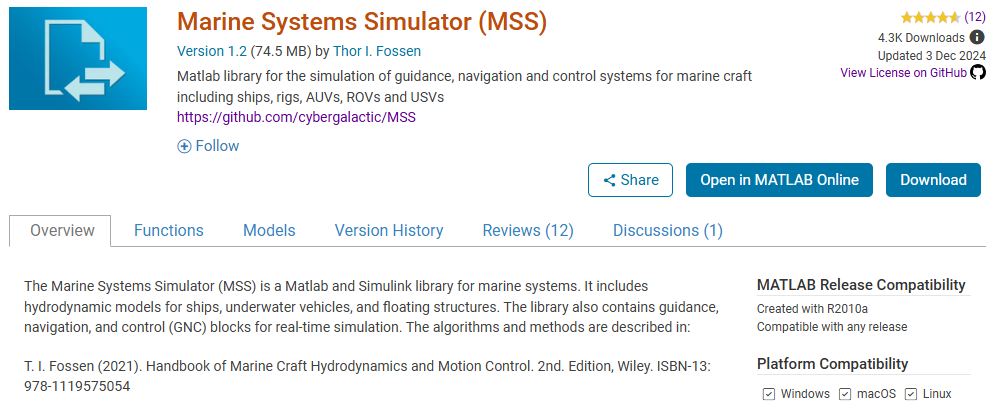
\includegraphics[width=0.7\linewidth]{img/mss toolbox.png}};
	\end{tikzpicture}
	
	\begin{tikzpicture}[remember picture,overlay]
		% \node[fill=blue!30, text=white, font=\large, rounded corners] 
		\node at (current page.north east) [xshift=-4.5cm, yshift=-6.5cm] 
		{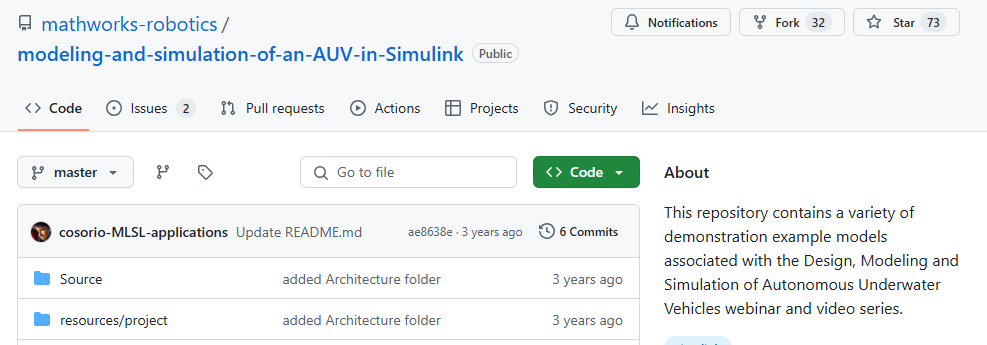
\includegraphics[width=0.7\linewidth]{img/simscape.png}};
	\end{tikzpicture}
	
	
	
	Marine Systems Simulator (MSS) Toolbox \footnote{T. I. Fossen and T. Perez (2004). Marine Systems Simulator (MSS). URL: https://github.com/cybergalactic/MSS} 
	
	\vspace{3cm}
	
	MATLAB Simscape Multibody \footnote{https://github.com/mathworks-robotics/modeling-and-simulation-of-an-AUV-in-Simulink} 
\end{frame}

% =========================================
% =========================================


\begin{frame}{Introduction}
	
	\begin{tikzpicture}[remember picture,overlay]
		% \node[fill=blue!30, text=white, font=\large, rounded corners] 
		\node at (current page.north east) [xshift=-3.8cm, yshift=-3cm] 
		{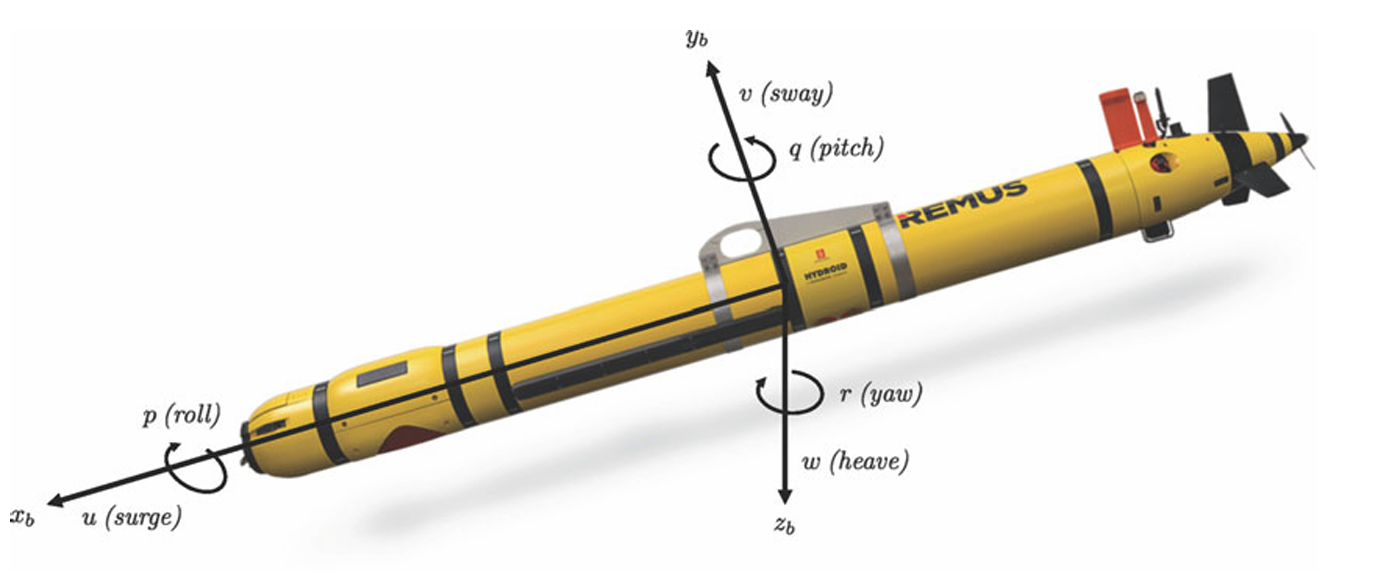
\includegraphics[width=0.7\linewidth]{img/6DOF motion AUV.png}};
	\end{tikzpicture}
	
	\vspace{2cm}
	
	Overview of this seminar
	\begin{itemize}
		\item Fundamental knowledge 
		\item 6-DOF model of a Rigid Body
		\item Ocean dynamics
		\item Environmental disturbances
		\item An example of the ODIN
		\item Guidance - Navigation - Control
		\item Numerical simulations
		\item Quasi-Physical Simulation for UV motion control
		\item An excample for GNC-integrated Quasi-Physical simulation
	\end{itemize}
\end{frame}




% =========================================
% =========================================
